% Ubah judul dan label berikut sesuai dengan yang diinginkan.
\section{Architecture}
\label{sec:arsitektur}

% Ubah paragraf-paragraf pada bagian ini sesuai dengan yang diinginkan.
In this study, a control device has been developed that can receive commands wirelessly from other devices such as a laptop or Jetson Nano. This subsection will detail the implementation of the device developed in this research.

Below are detailed some of the hardware and software used in this research, as follows:
\begin{enumerate}
    \item Anaconda Navigator
    \item Arduino IDE 
    \item Laptop 
    \item Jetson Nano
    \item Camera
    \item ESP32 Devkit V1
    \item 2 Motor Driver
    \item 2 DC-DC Voltage Regulator
    \item 2 DC Motor
    \item 24V Battery
\end{enumerate}

\subsection{Schematic}
\label{subsec:skematik alat}

The schematic of this device is illustrated in detail in Figure \ref{fig:Skematik Alat}. This system utilizes a camera connected to a laptop or Jetson Nano as the main device for capturing images. The workflow begins when the camera captures images of the object. These captured images are then processed by the laptop or Jetson Nano. In this system, a pre-programmed classification model plays a crucial role in interpreting the image data. The results of this classification process are crucial as they form the basis for determining the instruction codes to be implemented.

The instruction codes will then be combined with the maximum speed parameters previously set by the user. The combination of instruction codes and speed parameters will form a data package as wheelchair motion control. This data package will then be transmitted wirelessly, either via Bluetooth or WiFi, to the ESP32 Devkit V1 module.

The ESP32 plays a crucial role in controlling the wheelchair motor. The ESP32 will serve as the control center that receives the data package sent wirelessly by the user. Subsequently, the ESP32 will decode the data package and adjust the data into predefined variables. This data package decoding process will yield two main pieces of data, which will then be further processed by the ESP32.

The first variable is the direction variable, which plays a crucial role in determining the direction of movement for the wheelchair's two motors. This variable ensures that the motors move in the desired direction based on the received data. Additionally, there is the speed variable used to set the maximum speed of the motor movement.

In its implementation, there is a series of chained 'if' logics that will be detailed in the programming subsection. Simply put, this chained 'if' logic plays a crucial role in decision-making for both the direction and speed of the motors based on the received data. The result of this logic will provide triggers in the form of either 5V or 0V. This voltage will then influence the motor rotation direction.

Next, the speed variable will be used to adjust the Pulse Width Modulation (PWM) level on the motor controller. This PWM adjustment is crucial for controlling the motor rotation speed. By adjusting the PWM level, the maximum motor speed can be customized according to the requirements.

\begin{figure} [!ht] \centering
  % Nama dari file gambar yang diinputkan
  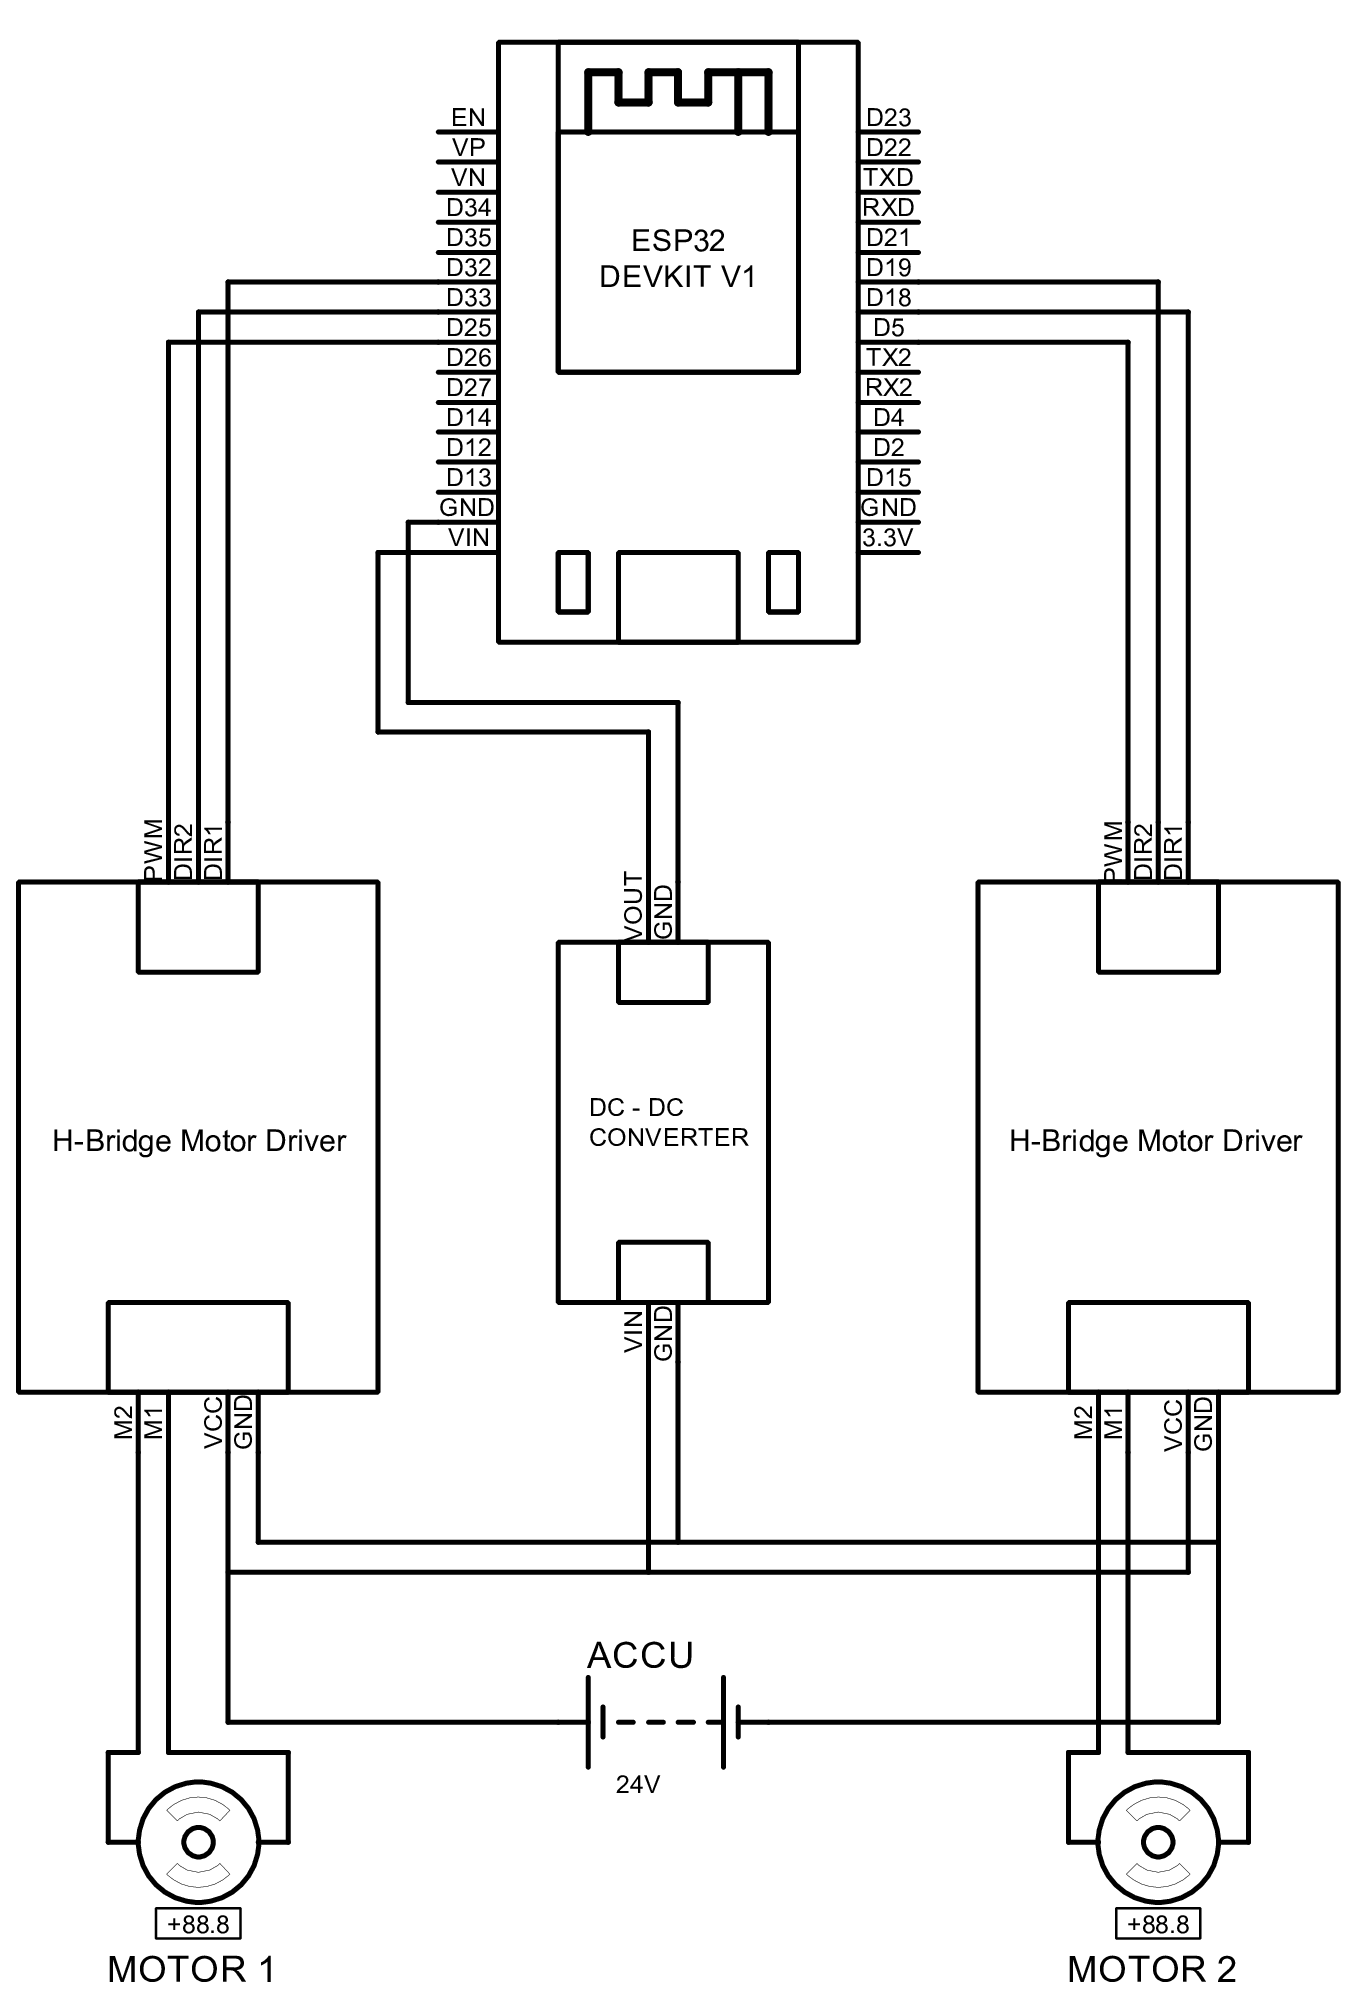
\includegraphics[scale=0.24]{gambar/bab3/Schematics.png}
  % Keterangan gambar yang diinputkan
  \caption{Schematic of the wheelchair motor control}
  % Label referensi dari gambar yang diinputkan
  \label{fig:Skematik Alat}
\end{figure}

